\section{Schwarzschild Black Holes}
Before examining what effects the more consequential features of black holes will have on orbital motion, the opportunity presents itself to build up an understanding in a much simpler environment than what will come up later.
Schwarzschild black holes -- the easier of the two to approach when compared to Kerr black holes -- possess no angular momentum and no electrical charge.
The lack of angular momentum is the more significant exclusion that is made here, as we do not need to worry about the orientation of the orbital motion relative to the black hole's axis of spin (or lack thereof).
Any orbits that travel clockwise about the black hole will follow an identical but mirrored path compared to another orbit that travels anti-clockwise around the black hole, with the same initial starting position and velocity, but a mirrored initial angle.
This symmetry about the $z$-plane is incredibly useful, particularly when visualising accretion disks, as only half of the problem needs to be solved directly, and then this portion of the work can be mirrored to complete it \cite{schwarzSymmetry}.
But why else is angular momentum such a significant factor to consider in these calculations?
Among other things, it can be shown that the difference between the innermost stable circular prograde orbit (the smallest stable circular orbit travelling \textit{with} the spin of the black hole) and the innermost stable circular retrograde orbit (the smallest stable circular orbit travelling \textit{against} the spin of the black hole) is substantial \cite{ISCOproret}.
This forces us to consider the orientation in which the mass is orbiting the black hole relative to its spin, and also sets strict lower and upper radial bounds on where stable circular orbits can exist. 

Turning to electric charge, why is this not close in significance to angular momentum regarding the role it plays in orbital motion?
As a rule, this parameter is set to zero under the assumption that for any charged black hole, the presence of plasmas around it will result in a discharging of this electric charge \cite{electricNegligence}.
Although this feature of black holes is not always ignored -- the Reissner-Nordstr{\"o}m metric deals with the case of zero angular momentum and non-zero electric charge, while the Kerr-Newman metric examines black holes with non-zero angular momentum and non-zero electric charge.
Furthermore, there are recent publications suggesting that researchers should not be so quick to ignore the effects of electric charge in black hole physics, and instead consider the effect it has on things such as the ISCO. \cite{electricNegligence}

\begin{figure}[!ht]
    \centering
    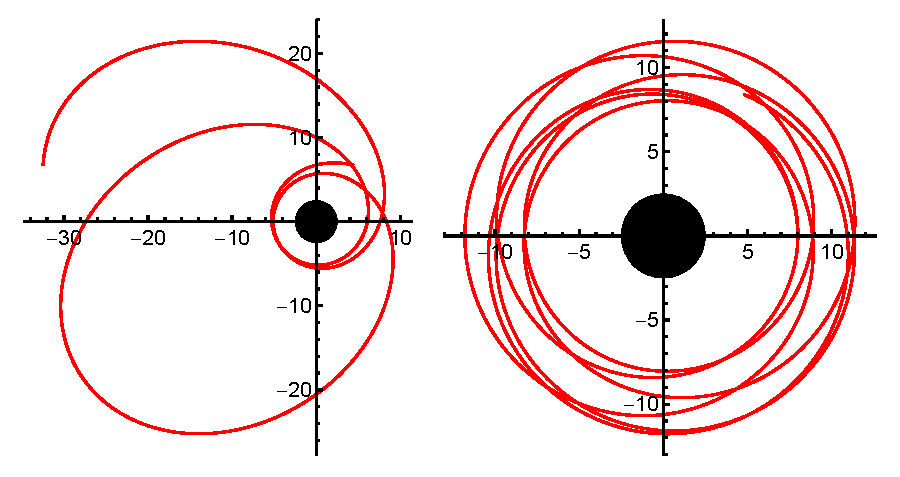
\includegraphics[width=0.8\textwidth]{images/schwarzSymmetry.pdf}
    \caption[Example of an eccentric and a comparatively far less eccentric Schwarzschild orbit]{A plot of an eccentric Schwarzschild orbit (left) with parameter values $E=0.976$, $L=3.842$, $r(t=0)=8$, and $M=1$, alongside a much less eccentric Schwarzchild orbit (right) with parameter values $E=0.956$, $L=3.74$, $r(t=0)=8$, and $M=1$.}
    \label{fig:symOrbits}
\end{figure}

%%%%%%%%%%%%%%%%%%%%%%%%%%%%%%%%%%%%%%%%%%%%%%%%%%%%%%%%%%%%%%%%%%%%%%%
%%%%%%%%%%%%%%%%%%%%%%%%%%   SECTION BREAK   %%%%%%%%%%%%%%%%%%%%%%%%%%
%%%%%%%%%%%%%%%%%%%%%%%%%%%%%%%%%%%%%%%%%%%%%%%%%%%%%%%%%%%%%%%%%%%%%%%

\subsection{Equations of Motion: Euler-Lagrange}
It is possible to derive the equations of motion for an orbiting test body using Lagrangian methods.
The Euler-Lagrange equation is defined as \cite{eulerLagrange}
\begin{equation}
\dv{\tau} \left(\frac{\partial \mathcal{L}}{\partial u^\alpha} \right)=\frac{\partial \mathcal{L}}{\partial x^\alpha}.
\end{equation}
Conventionally, we use the notation $x^\alpha$ to represent coordinates, where in this thesis $\alpha$ takes values in $\{t,r,\theta,\phi\}$.
We will use this $x^\alpha$ notation for formal definitions, but for everything else we shall use $x^\alpha\equiv\alpha$, where we note that $\alpha$ is a function of our coordinate time parameter, $t$, such that $\alpha\equiv\alpha(t)$.
The Lagrangian, $\mathcal{L}$, is \cite{chandraBook}
\begin{equation}\label{eqn:stdlagrangian}
2\mathcal{L}=g_{\alpha\beta}u^\alpha u^\beta,
\end{equation}
and $u^\alpha$ is the four-velocity
\begin{equation}
u^\alpha = \dv{x^\alpha}{\tau}.
\end{equation}
Here, $\tau$ represents our proper-time parameter, and the factor of $g_{\alpha\beta}$ in the Lagrangian is a metric, mentioned previously as part of the Christoffel symbols in Eqn.~\eqref{eqn:christoffel}.
This section of the paper is concerned with the Schwarzschild metric, which is defined as \cite{schwarz1916}
\begin{equation}\label{eqn:schwarzMet}
g_{\alpha\beta}=
\begin{pmatrix}
    -f(r) & 0 & 0 & 0\\
    0 & f(r)^{-1} & 0 & 0\\
    0 & 0 & r^2 & 0\\
    0 & 0 & 0 & r^2\sin(\theta)
\end{pmatrix},
\end{equation}
noting that we are using the $(-+++)$ signature, and define $f(r)$ as
\begin{equation}
f(r)=\frac{r-2M}{r}.
\end{equation}
Hereafter we use $f(r)\equiv f$ and understand, perhaps trivially, that $f^{-1}$ is defined to be the multiplicative inverse of $f$, so that $f\cdot f^{-1}=1$, and not the compositional inverse, in that $f^{-1}(f(r))=r$.
Expanding out our definition for the Lagrangian gives us $16$ terms in total, but only four of these will be non-zero due to the fact that any cross-terms $g_{\alpha\beta}$ such that $\alpha \neq \beta$ are equal to zero, specifically
\begin{align}
    2\mathcal{L}&=\left[\sum_{\alpha}g_{\alpha\alpha}(u^\alpha)^2\right]+\left[\sum_{\alpha\neq\beta}g_{\alpha\beta}u^\alpha u^\beta\right],\\
    &=\left[g_{tt}(u^t)^2+g_{rr}(u^r)^2+g_{\theta\theta}(u^\theta)^2+g_{\phi\phi}(u^\phi)^2\right]+\left[0\right],\\
    &=-f(u^t)^2+f^{-1}(u^r)^2+r^2(u^\theta)^2+r^2\sin^2(\theta)(u^\phi)^2.
\end{align}
Next, without loss of generality, the constraint of $\theta=\frac{\pi}{2}$ is introduced, fixing all orbits to remain in the equatorial plane, simplifying the system to a 3-dimensional problem in $t$, $r$, and $\phi$.
The Lagrangian then reduces to
\begin{align}
2\mathcal{L}&=-f(u^t)^2+f^{-1}(u^r)^2+r^2\cancelto{0}{(u^\theta)^2}+r^2(u^\phi)^2\cancelto{1}{\sin^2(\theta)},\\
&=-f(u^t)^2+f^{-1}(u^r)^2+r^2(u^\phi)^2 \label{eqn:reduclagran}.
\end{align}
The only coordinate dependency in the coefficients of $\{u^t, u^r, u^\phi\}$ is $r$, suggesting that examining the Euler-Lagrange equations for $\alpha=\{t,\phi\}$ may result in discovering constants of the system.
First, we calculate the equation for $\alpha=t$:
\begin{align}
    \dv{}{\tau}\left(\dv{(2\mathcal{L})}{u^t} \right)&=\pdv{(2\mathcal{L})}{t},\\
    \dv{}{\tau}\left(\dv{}{u^t}\left( -f(u^t)^2+f^{-1}(u^r)^2+r^2(u^\phi)^2\right) \right)&=\pdv{}{t}\left( -f(u^t)^2+f^{-1}(u^r)^2+r^2(u^\phi)^2\right),\\
    \dv{}{\tau}\left[2(-fu^t) \right]&=0,\\
    \Rightarrow -fu^t&=E. \label{eqn:tConstantEuler}
\end{align}
This first constant is invariant with regards to time translation, and so we define it to be the energy, $E$ \cite{introCondensed}, of the test body as measured by a stationary asymptotic observer, that is, a stationary observer far enough away from the black hole that its effects on said observer can be ignored.
Reorganising Eqn.~\eqref{eqn:tConstantEuler} to the following form to better represent the goal of these calculations gives us
\begin{equation}\label{eqn:ut}
u^t=-\frac{E}{f}.
\end{equation}
Next, we calculate the Euler-Lagrange equation for $\alpha=\phi$,
\begin{align}
    \dv{}{\tau}\left(\dv{(2\mathcal{L})}{u^\phi} \right)&=\pdv{(2\mathcal{L})}{\phi},\\
    \dv{}{\tau}\left(\dv{}{u^\phi}\left( -f(u^t)^2+f^{-1}(u^r)^2+r^2(u^\phi)^2\right) \right)&=\pdv{}{\phi}\left( -f(u^t)^2+f^{-1}(u^r)^2+r^2(u^\phi)^2\right),\\
    \dv{}{\tau}\left[2(r^2u^\phi) \right]&=0,\\
    \Rightarrow r^2u^\phi&=L. \label{eqn:phiConstantEuler}
\end{align}
This second constant is invariant with regards to rotation, and so is defined as the angular momentum, $L$ \cite{introCondensed}, of the test body as measured by a stationary asymptotic observer.
Again, rearranging Eqn.~\eqref{eqn:phiConstantEuler} to better represent the goal of these calculations gives us
\begin{equation}\label{eqn:uphi}
    u^\phi=\frac{L}{r^2}.
\end{equation}
Substituting Eqns.~\eqref{eqn:ut} and \eqref{eqn:uphi} back into Eqn.~\eqref{eqn:reduclagran} gives us
\begin{equation}\label{eqn:prefinaldrdt2}
-\frac{E^2}{f}+f^{-1}(u^r)^2+\frac{L^2}{r^2}=-1,
\end{equation}
where normalising the equation to $-1$ comes from the need to make the equations \textit{timelike}.
Specifically, we are normalising the four-velocity,
\begin{equation}\label{eqn:fourvelocity}
u^\alpha u_\alpha=c^2,
\end{equation}
so that $c^2=-1$, to signify that the test body is travelling along a timelike geodesic.
The other common option is to set $c^2=0$ in Eqn.~\eqref{eqn:fourvelocity}, which signifies that the test body is travelling along a \textit{null} geodesic -- this is used with massless particles like photons.
Rearranging Eqn.~\eqref{eqn:prefinaldrdt2} we get
\begin{equation}\label{eqn:drdt2}
\left(\dv{r}{\tau}\right)^2=E^2-f(r)\left(1+\frac{L^2}{r^2}\right).
\end{equation}
This equation can be manipulated to give us the following set of equations:
\begin{align}
    \dv[2]{r}{\tau}&=L(r^{-3}-3r^{-4})-r^{-2},\label{eqn:geodr2dt2}\\
    \dv{r}{\tau}&=\pm\sqrt{E^2-f(r)\left(1+\frac{L^2}{r^2}\right)},\label{eqn:geodrdt} \\
    u^r(0)&=\left.\dv{r}{\tau}(0)\right|_{\tau=0},\label{eqn:geour0}
\end{align}
where Eqn.~\eqref{eqn:geodr2dt2} is solved numerically using Eqn.~\eqref{eqn:geodrdt} and Eqn.~\eqref{eqn:geour0} as initial conditions. This concludes the first method of solving for the equations of motion.

%%%%%%%%%%%%%%%%%%%%%%%%%%%%%%%%%%%%%%%%%%%%%%%%%%%%%%%%%%%%%%%%%%%%%%%
%%%%%%%%%%%%%%%%%%%%%%%%%%   SECTION BREAK   %%%%%%%%%%%%%%%%%%%%%%%%%%
%%%%%%%%%%%%%%%%%%%%%%%%%%%%%%%%%%%%%%%%%%%%%%%%%%%%%%%%%%%%%%%%%%%%%%%

\subsection{Equations of Motion: Geodesic}
Moving on, the second method makes use of the geodesic equations as defined in Eqn.~\eqref{eqn:geodesic_eqn}.
Similar to the Euler-Lagrange method, we begin with the Schwarzschild metric, as defined in Eqn.~\eqref{eqn:schwarzMet}, and calculate the Lagrangian from Eqn.~\eqref{eqn:stdlagrangian}.
We may rescale the affine parameter $\tau$ so that $2\mathcal{L}=-1$, this is again done by setting $c^2=-1$ in the four-velocity definition from Eqn.~\eqref{eqn:fourvelocity}.
Without loss of generality we also set the values $\theta(t=0)=\pi/2$ and $u^{\theta}(t=0)=0$ to ensure the orbit remains in the equatorial plane.
Explicitly, at $t=0$, we use the notation $\alpha(t=0)\equiv\alpha_0$ and $u^\alpha(t=0)=u_0^\alpha$. The Lagrangian $2\mathcal{L}=-1$ evaluates to
\begin{gather}
    -f\vert_{r_0}(u_0^t)^2+f^{-1}\vert_{r_0}(u_0^r)^2-r_0^2(u_0^\phi)^2=-1,\\
    -\left(1-\frac{2M}{r_0}\right)(u_0^t)^2 +\frac{r_0}{r_0-2M}(u_0^r)^2-r_0^2(u_0^\phi)^2=-1. \label{eqn:secordLag}
\end{gather}
Now Eqn.~\eqref{eqn:secordLag} is solved for $u_0^{r}$ to give us
\begin{equation}
u_0^r=\frac{r_0-2M}{r_0}\left[\left(1-\frac{2M}{r_0}\right)(u_0^t)^2+r_0(u_0^\phi)^2-1 \right].
\end{equation}
This is the final initial condition needed before numerically solving the geodesic equations for $r$ and $\phi$ over a determined timeframe, where the initial values of $r_0$ and $u_0^\phi$ are set manually and we take $M=1$.
The system to be solved then becomes
\begin{align}
        \dv[2]{x^t}{\lambda}+\Gamma^{t}{}_{\beta\delta}\dv{x^\beta}{\lambda}\dv{x^\delta}{\lambda}=0,\\
        \dv[2]{x^r}{\lambda}+\Gamma^{r}{}_{\beta\delta}\dv{x^\beta}{\lambda}\dv{x^\delta}{\lambda}=0,\\
        \dv[2]{x^\phi}{\lambda}+\Gamma^{\phi}{}_{\beta\delta}\dv{x^\beta}{\lambda}\dv{x^\delta}{\lambda}=0,
\end{align}
where $\{\beta,\delta\}$ takes values in $\{t,r,\theta,\phi\}$.
This concludes our second method for solving for the equations of motion. 

Looking at Fig.~\eqref{fig:matchedOrbits}, we see a plot of the Euler-Lagrange method for solving for the equations of motion.
Along with this, there are also plots of the radial and angular errors between both the Euler-Lagrange and the Geodesic methods.
It can be seen that for small values of $\tau$ there is comparatively little error relative to the full timeframe -- resulting in almost identical plots.
This test on both derivations has shown that both methods are correct and allows for confidence in any future results where either of these methods will be used to derive and plot orbits.
The error for larger values of $\tau$ begins to spike at approximately the same point on both plots, around some critical value $\tau_c\approx 375$.
This is a truncation error that is being accumulated from as early $\tau=0$ in the ODE solver, as is natural in numerical solutions when two different methods are used, but it seems to grow rapidly beyond $\tau=\tau_c$.
As these plots and calculations were carried out in Mathematica, the easiest way to reduce this error would be to deliberately force Mathematica to carry out these calculations to a greater number of significant figures.

\begin{figure}[!ht]
    \centering
    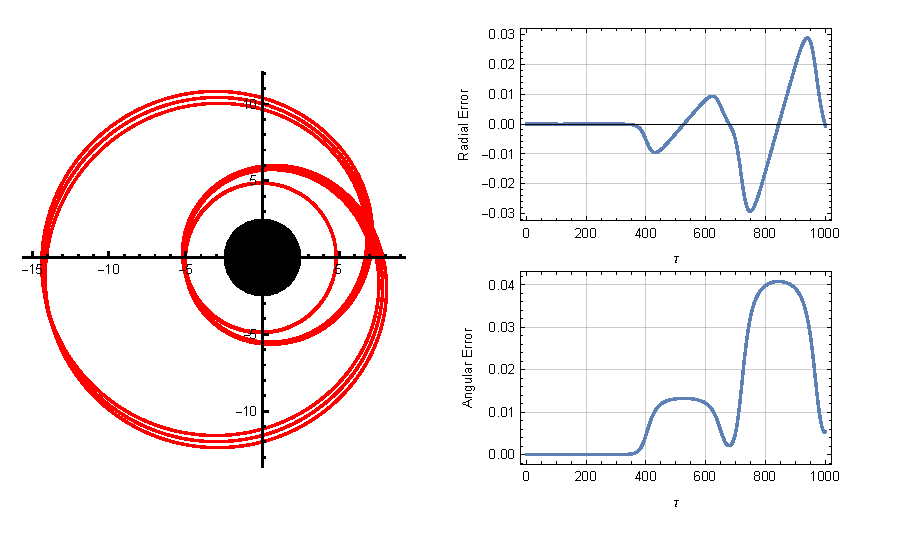
\includegraphics[width=\textwidth]{images/MatchedOrbits.pdf}
    \caption[Matched orbits: Euler-Lagrange and Geodesic Equations]{A plot of the equations of motion when solved for using the Euler-Lagrange method (left) and the errors when comparing the radial values (upper-right) and angular values (lower-right) between the Euler-Lagrange method and the Second-Order Geodesic method. It can be seen that both methods produce identical results (within reasonable precision). The parameter values for this plot are $E=\sqrt{217/237}$, $L=72/\sqrt{395}$, $M=1$, $r_0=7.2$.}
    \label{fig:matchedOrbits}
\end{figure}

%%%%%%%%%%%%%%%%%%%%%%%%%%%%%%%%%%%%%%%%%%%%%%%%%%%%%%%%%%%%%%%%%%%%%%%
%%%%%%%%%%%%%%%%%%%%%%%%%%   SECTION BREAK   %%%%%%%%%%%%%%%%%%%%%%%%%%
%%%%%%%%%%%%%%%%%%%%%%%%%%%%%%%%%%%%%%%%%%%%%%%%%%%%%%%%%%%%%%%%%%%%%%%

\subsection{Bound Orbits}
Now that a general method for calculating and plotting orbits about Schwarzschild black holes has been established, an important step from here would be to understand the conditions and situations in which \textit{bound} orbits occur.
Using Eqn.~\eqref{eqn:drdt2} we may infer that the effective potential of the system is
\begin{equation}\label{eqn:effPot}
    V(L,r)=f(r)\left(1+\frac{L^2}{r^2}\right).
\end{equation}
This equation has been plotted in Fig.~\eqref{fig:radEffPot}, and from here we notice a number of features about the effective potential and closely follow the work done by Cutler et al. \cite{cutlerEtAl} in examining them.
Expanding the equation $E^2=V(L,r)$ gives us
\begin{equation}\label{eqn:cubicEffPot}
    (1-E^2)r^3-2Mr^2+L^2r-2ML^2=0,
\end{equation}
a cubic with three roots $r_1$, $r_2$, and $r_3$ (for the purposes of the graphic in Fig.~\eqref{fig:radEffPot}, $E$ and $L$ have been chosen so that the roots are distinct).
By convention, the roots are ordered $r_1<r_2<r_3$, and are used to classify three types of orbits.
For radii $r<r_1$ we have plunging orbits, which will tend towards the black hole due to the increased strength of its pull which is caused by the test body's proximity to it.
For radii $r_2<r<r_3$ and $E<1$ we have bound orbits, the specific behaviours of these orbits may vary, but they will neither escape the black hole's pull nor plunge directly into it.
Finally, for $E\geq 1$ we have escaping orbits, where $r_3\rightarrow \infty$ as there is not enough pull from the black hole to keep the orbit close to it, and it will shoot away.
Although in Fig.~\eqref{fig:radEffPot}, for the line $E_\text{bound}$ we cannot have values of $r>r_3$, nor can we have values of $r$ such that $r_1<r<r_2$.
Recalling Eqn.~\eqref{eqn:geodrdt}, any of the previously mentioned disallowed values of $r$ would give
\begin{gather}
    E^2<f\left(1+\frac{L^2}{r^2}\right)=V(L,r),\\
    \Rightarrow E^2-V(L,r)<0,\\
    \Rightarrow \sqrt{E^2-V(L,r)} \in \mathbb{C},\\
    \dv{r}{\tau}\in\mathbb{C}.
\end{gather}
Complex values of radial velocity do not make physical sense, and so the values of $r$ that produce them are not considered.

There are two other lines of interest to consider apart from $E_\text{bound}$, where ``extremal" behaviours of the orbit can be discussed.
Beginning with $E_\text{circular}$, this corresponds to the value of $E$ such that $r_2=r_3$ and produces a stable circular orbit.
For $E\gtrapprox E_\text{circular}$, any perturbation away from this point will not cause the orbit to change, and instead it will return to its state pre-perturbation.
The line $E_\text{unstable}$ corresponds to $r_1=r_2$, and in contrast to the $E_\text{circular}$ case, \textit{any} perturbation from this point will cause the orbit to either plunge into the black hole or scatter off into space.

\begin{figure}[!ht]
    \centering
    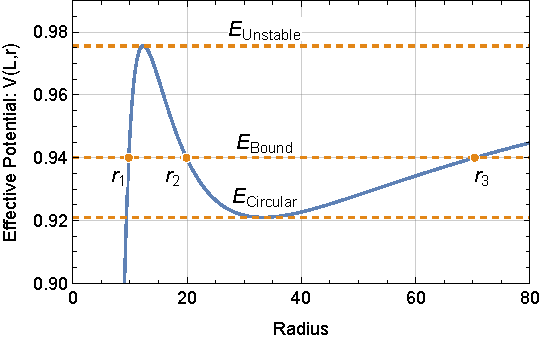
\includegraphics{images/RadialPotentialPE.pdf}
    \caption[Schwarzschild radial effective potential plot]{A plot of the radial effective potential where, depending on the magnitude of the energy, plunging orbits are found at $r<r_1$, bound motion is found at $r_2<r<r_3$, and escaping orbits are found at $r>r_3$.}
    \label{fig:radEffPot}
\end{figure}

%%%%%%%%%%%%%%%%%%%%%%%%%%%%%%%%%%%%%%%%%%%%%%%%%%%%%%%%%%%%%%%%%%%%%%%
%%%%%%%%%%%%%%%%%%%%%%%%%%   SECTION BREAK   %%%%%%%%%%%%%%%%%%%%%%%%%%
%%%%%%%%%%%%%%%%%%%%%%%%%%%%%%%%%%%%%%%%%%%%%%%%%%%%%%%%%%%%%%%%%%%%%%%

\subsection{Parameterisation: $p$-$e$}
Up until this point, any discussion regarding orbital motion and types of orbits has revolved around the values of $E$ and $V(L,r)$, or, more explicitly, the two independent constants $E$ and $L$.
These values do not give us a tangible understanding of the type of orbit being analysed.
Thus, two parameters are introduced; the \textit{semi-latus rectum}, $p$, and the \textit{eccentricity}, $e$, which, as mentioned in Sec.~\eqref{sec:introduction}, correspond to the size and non--circularity of the orbit respectively.
The derivation and implementation of these parameters closely follows the work done by Cutler et al. \cite{cutlerEtAl}.
When the values of $E$ and $L$ satisfy the requirements so that bound orbital motion is achieved, the following equation holds
\begin{equation}
    f(r)\left(1+\frac{L^2}{r^2}\right)=E^2.
\end{equation}
This equation can be expanded to give Eqn.~\eqref{eqn:cubicEffPot}, where the roots of this equation are the $r_i$ values seen in Fig.~\eqref{fig:radEffPot} as before.
The two parameters $p$ and $e$ can then be defined as satisfying
\begin{gather}
		r_{\text{max}}=\frac{pM}{1-e},\label{eqn:rmax}\\
        r_{\text{min}}=\frac{pM}{1+e},\label{eqn:rmin}
\end{gather}
with $r_\text{min}=r_2$ and $r_\text{max}=r_3$.
From this, using Eqn.~\eqref{eqn:cubicEffPot} and comparing it to the standard form of a cubic equation $(r-r_1)(r-r_2)(r-r_3)=0$, we may also deduce
\begin{gather}
r_1=\frac{2pM}{p-4},\\
E^2=\frac{(p-2-2e)(p-2+2e)}{p(p-3-e^2)},\\
L^2=\frac{p^2M^2}{p-3-e^2}.
\end{gather}

\begin{figure}
    \centering
    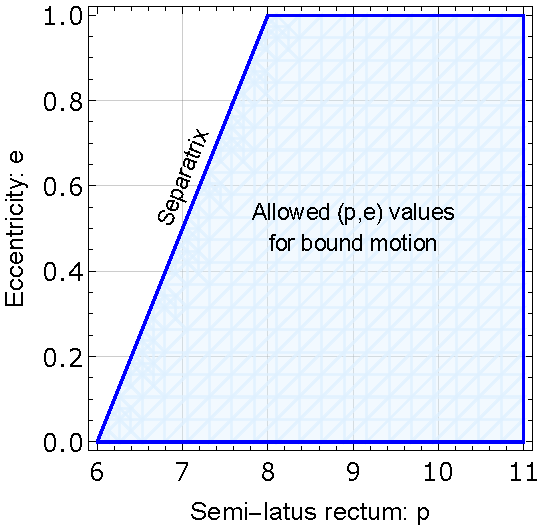
\includegraphics[width=0.4\textwidth]{images/PEPlane.pdf}
    \caption[Plot of $(p,e)$-plane with separatrix]{A plot of the $(p,e)$ plane showing all of the values of $p$ and $e$ which produce bound orbits, and the separatrix.}
    \label{fig:PEPlane}
\end{figure}
\noindent
Now it is possible to develop some understanding about different types of orbits from intuition regarding the values of $p$ and $e$.
For example, \textit{stable} circular orbits, corresponding to the line $E_\text{circular}$ in Fig.~\eqref{fig:radEffPot}, require that $r_2=r_3$, which gives
\begin{align}
    \frac{pM}{1+e}&=\frac{pM}{1-e},\\
    \Rightarrow e&=0.
\end{align}
\noindent
\textit{Unstable} circular orbits, corresponding to the line $E_\text{unstable}$, require that $r_1=r_2$, which gives
\begin{align}
    \frac{2pM}{p-4}&=\frac{pM}{1+e},\\
    p-4&=2(1+e),\\
    \Rightarrow p&=6+2e.
\end{align}
To expand on this, for any values $p<6+2e$ we would obtain a plunging orbit, meaning that we can establish a domain of possible values in order to obtain bound orbits, as seen in Fig.~\eqref{fig:PEPlane}.
In this figure, the leftmost line, $p=6+2e$, is known as the \textit{separatrix} -- this line separates the region of the parameter space corresponding to stable orbits from the region corresponding to unstable or plunging orbits \cite{nielsLastStableOrbit}.\\

%%%%%%%%%%%%%%%%%%%%%%%%%%%%%%%%%%%%%%%%%%%%%%%%%%%%%%%%%%%%%%%%%%%%%%%
%%%%%%%%%%%%%%%%%%%%%%%%%%   SECTION BREAK   %%%%%%%%%%%%%%%%%%%%%%%%%%
%%%%%%%%%%%%%%%%%%%%%%%%%%%%%%%%%%%%%%%%%%%%%%%%%%%%%%%%%%%%%%%%%%%%%%%

\subsection{Parameterisation: Darwin}
In wishing to obtain the frequencies of orbit, we will need to integrate Eqns.~\eqref{eqn:uphi} and \eqref{eqn:drdt2}.
Since we do not know the period of $\tau$ before carrying out these calculations, it is desirable to eliminate it as the variable of integration and instead use $r$.
This is done in the following way by, again, closely following the work by Cutler et al. \cite{cutlerEtAl}.
We note from Eqn.~\eqref{eqn:geodrdt} that
\begin{equation}
\dv{r}{\tau}=\sqrt{E^2-V},
\end{equation}
where $V\equiv V(L,r)$ is defined as is Eqn.~\eqref{eqn:effPot}.
Hence, using the chain rule, we get
\begin{align}
    \dv{t}{r}&=\dv{t}{\tau}\dv{\tau}{r},\\
    &=\left(-\frac{E}{f} \right)\left(\frac{1}{\sqrt{E^2-V}} \right),\\
    \intertext{and}
    \dv{\phi}{r}&=\dv{\phi}{\tau}\dv{\tau}{r},\\
    &=\left(\frac{L}{r^2}\right)\left(\frac{1}{\sqrt{E^2-V}} \right).
\end{align}
Unfortunately, this is not enough to carry out our desired calculations -- since $r$ is multi-valued along the path of integration we will need to split the path into two parts.
To avoid this we introduce Darwin's parameter, $\chi$, which is defined as 
\begin{equation}\label{eqn:darwinparam}
r(\chi)=\frac{pM}{1+e\cos(\chi)},
\end{equation}
where $\chi$ ranges from $0$ to $2\pi$.
Now instead of integrating with respect to $r$ it is more desirable to integrate with respect to $\chi$ as, unlike $r$, it is single-valued along the path on integration.
Using the chain rule we may utilise Eqn.~\eqref{eqn:darwinparam} in the following way:
\begin{equation}
\dv{t}{\chi}=\dv{t}{\tau}\dv{\tau}{r}\dv{r}{\chi}.
\end{equation}
Term-by-term we get
\begin{align}
\dv{t}{\tau}&=\left(\frac{p}{p-2-2e\cos(\chi)} \right)\left(\frac{(p-2-2e)(p-2+2e)}{p(p-3-e^2)}\right),\\
\dv{\tau}{r}&=\left(e^2\sin^2(\chi)\left(\frac{p-6-2e\cos(\chi)}{p(p-3-e^2)} \right)\right)^{-\frac{1}{2}},\\
\dv{r}{\chi}&=\left(\frac{pMe\sin(\chi)}{(1+e\cos(\chi))^2} \right),
\end{align}
where a more thorough derivation of these terms can be seen in Appendix \ref{apx:darwin}. Hence,
\begin{align}
\begin{split}
\dv{t}{\chi}&=\left(\frac{p}{p-2-2e\cos(\chi)} \right)\left(\frac{(p-2-2e)(p-2+2e)}{p(p-3-e^2)}\right)\\
&\qquad\times\left(e^2\sin^2(\chi)\left(\frac{p-6-2e\cos(\chi)}{p(p-3-e^2)} \right)\right)^{-\frac{1}{2}}\\
&\qquad\times\left(\frac{pMe\sin(\chi)}{(1+e\cos(\chi))^2} \right),
\end{split}
\end{align}
and therefore,
\begin{equation}\label{eqn:dtdchi}
\begin{split}
\dv{t}{\chi}&=p^2M(p-2+2e)^{\frac{1}{2}}(p-2-2e)^{\frac{1}{2}}(p-2-2e\cos(\chi))^{-1}\\
&\qquad\times(p-6-2e\cos(\chi))^{-\frac{1}{2}}(1+e\cos(\chi))^{-2}.
\end{split}
\end{equation}
We also see that 
\begin{equation}
\dv{\phi}{\chi}=\dv{\phi}{\tau}\dv{\tau}{r}\dv{r}{\chi},
\end{equation}
where the latter two terms are the same as before, while the first term is known to be
\begin{equation}
\dv{\phi}{\tau}=\frac{L}{r^2}=\left(\frac{p^2M^2}{p-3-e^2} \right)^{\frac{1}{2}}\left(\frac{1+e\cos(\chi)}{pM} \right)^2.
\end{equation}
After substitution we get
\begin{align}
    \dv{\phi}{\chi}&=\left(\frac{L}{r^2}\right)\left(e^2\sin^2(\chi)\left(\frac{p-6-2e\cos(\chi)}{p(p-3-e^2)}\right)\right)^{-\frac{1}{2}}\left(\frac{pMe\sin(\chi)}{(1+e\cos(\chi))^2} \right)\\
    \begin{split}
    &=\left(\left(\frac{p^2M^2}{p-3-e^2} \right)\left(\frac{1+e\cos(\chi)}{pM} \right)^2\right)\left(\frac{(p(p-3-e^2))^{\frac{1}{2}}}{e\sin(\chi)(p-6-2e\cos(\chi))^{\frac{1}{2}}} \right)\\
    &\qquad\times\left(\frac{pMe\sin(\chi)}{(1+e\cos(\chi))^2} \right),
    \end{split}
\end{align}
and hence,
\begin{equation}\label{eqn:dphidchi}
	\dv{\phi}{\chi}=\left(p(p-6-2e\cos(\chi))^{-1}\right)^{\frac{1}{2}}.
\end{equation}
%%%%%%%%%%%%%%%%%%%%%%%%%%%%%%%%%%%%%%%%%%%%%%%%%%%%%%%%%%%%%%%%%%%%%%%
%%%%%%%%%%%%%%%%%%%%%%%%%%   SECTION BREAK   %%%%%%%%%%%%%%%%%%%%%%%%%%
%%%%%%%%%%%%%%%%%%%%%%%%%%%%%%%%%%%%%%%%%%%%%%%%%%%%%%%%%%%%%%%%%%%%%%%

\subsection{Frequencies: Coordinate Time}
Moving forward with our derivation of orbital frequencies, it is now straightforward to define the following equations by integrating Eqns.~\eqref{eqn:dtdchi} and \eqref{eqn:dphidchi}:
\begin{equation}
\begin{split}
t(\chi)&=p^2M(p-2+2e)^{\frac{1}{2}}(p-2-2e)^{\frac{1}{2}}\\
&\qquad\times\int_0^\chi\left[(p-2-2e\cos(\chi'))^{-1}(p-6-2e\cos(\chi'))^{-\frac{1}{2}}(1+e\cos(\chi'))^{-2}\right]\dd{\chi'},\\
\end{split}
\end{equation}
and
\begin{equation}
\phi(\chi)=p^{\frac{1}{2}}\int_0^\chi\left[\frac{1}{\sqrt{p-6-2e\cos(\chi')}}\right]\dd{\chi'}.
\end{equation}
Performing the substitution $\chi \rightarrow 2\psi-\pi$, the integral $\phi(2\pi)$ becomes a complete elliptic integral of the first kind, so that
\begin{equation}
\phi(2\pi)=4\left(\frac{p}{p-6+2e} \right)^{\frac{1}{2}}K\left(\frac{4e}{p-6+2e}\right),
\end{equation}
with
\begin{equation}\label{eqn:ellipticintegral}
    K(x)\coloneqq \int_{0}^{\frac{\pi}{2}}\frac{\dd{\theta}}{\sqrt{1-x\sin^2(\theta)}}.
\end{equation}
It is now possible to calculate values for the radial period and $\Delta\phi=\phi(2\pi)$.
From here, the \textit{radial frequency} is defined as 
\begin{equation}\label{eqn:radfreqdar}
\Omega_r=\frac{2\pi}{t(2\pi)},
\end{equation}
and the \textit{azimuthal frequency} is
\begin{equation}\label{eqn:phifreqdar}
\Omega_\phi=\frac{\phi(2\pi)}{2\pi}\Omega_r.
\end{equation}
The fact that these frequencies are different is a sign of precession.
In Newtonian relativity we do not have precession, but, as mentioned at the beginning of Sec.~\eqref{sec:motivation}, through general relativity the precession of Mercury was discovered, and through analysis of its orbital frequencies it's exact perihelion shift was calculated \cite{mercuryPrecess}.

%%%%%%%%%%%%%%%%%%%%%%%%%%%%%%%%%%%%%%%%%%%%%%%%%%%%%%%%%%%%%%%%%%%%%%%
%%%%%%%%%%%%%%%%%%%%%%%%%%   SECTION BREAK   %%%%%%%%%%%%%%%%%%%%%%%%%%
%%%%%%%%%%%%%%%%%%%%%%%%%%%%%%%%%%%%%%%%%%%%%%%%%%%%%%%%%%%%%%%%%%%%%%%

\section{Kerr Black Holes}
\begin{figure}
\centering
    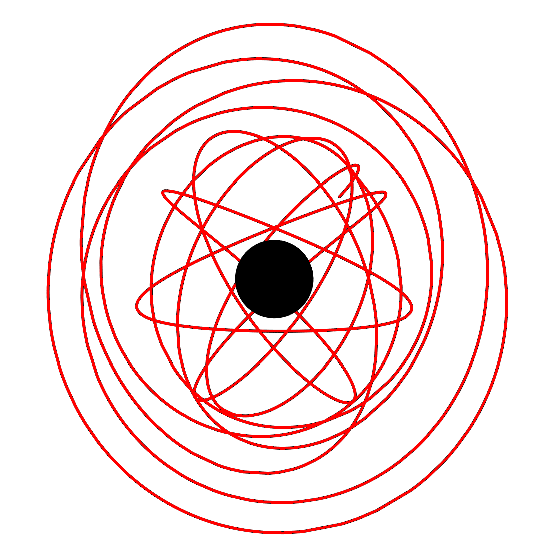
\includegraphics[width=0.4\textwidth]{images/KerrOrbitExample1.pdf}
    \caption[Kerr black hole example]{A plot of a path traced out by an orbit about a Kerr black hole. The parameter values for this plot are $a=0.7$, $p=4.93$, $e=0.3$, $x=0.5$.}
    \label{fig:kerrExample}
\end{figure}
The line element of the Kerr metric is defined as the following \cite{Teukolsky_2015}:
\begin{equation}\label{eqn:kerrmetric}
\begin{split}
\dd{s}^2&=-\left(1-\frac{2Mr}{\Sigma} \right)\dd{t}^2 + \frac{\Sigma}{\Delta}\dd{r}^2 +\Sigma\dd{\theta}^2+\left(r^2+a^2+\frac{2Ma^2r\sin^2(\theta)}{\Sigma}\right)\sin^2(\theta)\dd{\phi}^2\\
 &\qquad- \frac{4Mar\sin^2(\theta)}{\Sigma}\dd{t}\dd{\phi},
\end{split}
\end{equation}
where $M$ and $L=aM$ are the mass and angular momentum respectively, and
\begin{gather}
	\Delta=r^2-2Mr+a^2,\\
    \Sigma=r^2+a^2z^2,\\
    z=\cos(\theta).
\end{gather}
From this, the black hole is now bestowed with angular momentum, adding another layer of consideration when examining orbits about it.
Unlike the Schwarzschild case, the \textit{direction} in which a body is travelling relative to the black hole must be taken into account.
Test bodies travelling with the direction of the black hole's angular momentum will be able to obtain a stable circular orbit closer to the event horizon than those travelling against it.
In moving to the Kerr metric, orbits outside of the equatorial plane are now examined, so we may now examine orbits such as those in Fig.~\eqref{fig:kerrExample}.
These orbits are solved numerically using the Mathematica package titled ``KerrGeodesics", which is part of the ``Black Hole Perturbation Toolkit", where within this toolkit there are functions for computing separatrix values, frequencies, and resonances.

%%%%%%%%%%%%%%%%%%%%%%%%%%%%%%%%%%%%%%%%%%%%%%%%%%%%%%%%%%%%%%%%%%%%%%%
%%%%%%%%%%%%%%%%%%%%%%%%%%   SECTION BREAK   %%%%%%%%%%%%%%%%%%%%%%%%%%
%%%%%%%%%%%%%%%%%%%%%%%%%%%%%%%%%%%%%%%%%%%%%%%%%%%%%%%%%%%%%%%%%%%%%%%

\subsection{Parameterisation: Mino}
The general form for the radial and polar equations of motion in the Kerr metric are as follows \cite{resoFujita}:
\begin{align}
    \Sigma^2\left(\dv{r}{\tau}\right)^2&=R(r),\label{eqn:kerrRadial}\\
    \Sigma^2\left(\dv{z}{\tau}\right)^2&=\Theta(z),\label{eqn:kerrPolar}
\end{align}
where
\begin{align}
    R(r)&=[E(r^2+a^2)-aL_z]^2-\Delta(r^2+(aE-L_z)^2+Q),\\
    \Theta(z)&=Q-(Q+a^2(1-E^2)+L^2_z)z^2+a^2(1-E^2)z^4.
\end{align}
Here $Q$ is defined as the Carter constant \cite{carterDefinition}.
The $\Sigma^2$ term in Eqns.~\eqref{eqn:kerrRadial} and \eqref{eqn:kerrPolar} causes them to be coupled, they may be decoupled through the introduction of \textit{Mino time parameterisation}.
The Mino parameter $\lambda=\int \dd{\tau}/\Sigma=\int \dd{\tau}/(r^2+a^2z^2)$ may be rewritten as
\begin{equation}
\dv{\lambda}{\tau}=\frac{1}{\Sigma},
\end{equation}
and therefore, the following terms may also be rewritten as
\begin{align}
\dv{r}{\tau}&=\dv{r}{\lambda}\dv{\lambda}{\tau}=\dv{r}{\lambda}\frac{1}{\Sigma},\\
\dv{z}{\tau}&=\dv{z}{\lambda}\dv{\lambda}{\tau}=\dv{z}{\lambda}\frac{1}{\Sigma}.
\end{align}
Hence, Eqns.~\eqref{eqn:kerrRadial} and \eqref{eqn:kerrPolar} become decoupled through the following substitution:
\begin{align}
    \Sigma^2\left(\dv{r}{\tau}\right)^2&=\Sigma^2\left(\dv{r}{\lambda}\frac{1}{\Sigma} \right)\quad \Rightarrow \quad \left(\dv{r}{\lambda} \right)^2=R(r),\\
    \Sigma^2\left(\dv{z}{\tau}\right)^2&=\Sigma^2\left(\dv{z}{\lambda}\frac{1}{\Sigma} \right)\quad \Rightarrow \quad\left(\dv{z}{\lambda} \right)^2=\Theta(z).
\end{align}
The radial equation and polar equation are now purely functions of their respective coordinates, $r$ and $\theta$, but they are also now parameterised by the Mino parameter $\lambda$.

%%%%%%%%%%%%%%%%%%%%%%%%%%%%%%%%%%%%%%%%%%%%%%%%%%%%%%%%%%%%%%%%%%%%%%%
%%%%%%%%%%%%%%%%%%%%%%%%%%   SECTION BREAK   %%%%%%%%%%%%%%%%%%%%%%%%%%
%%%%%%%%%%%%%%%%%%%%%%%%%%%%%%%%%%%%%%%%%%%%%%%%%%%%%%%%%%%%%%%%%%%%%%%

\subsection{Frequencies: Mino Time}
Upon introduction of the Mino time parameter, it is now natural to define our frequencies in terms of it.
The $r$ and $\theta$ frequencies are of particular interest for the remainder of this thesis as they will constitute the foundation of the final section -- resonant orbits.
Closely following the work done by Warburton, Barack, and Sago \cite{warburtonKerrGeodesics}, we note that upon decoupling Eqns.~\eqref{eqn:kerrRadial} and \eqref{eqn:kerrPolar} they become inherently periodic with frequencies $\Upsilon_r$ and $\Upsilon_\theta$.
The frequency $\Upsilon_\phi$, although not discussed here, can be found through an infinite-time-average of $\dd{\phi}/\dd{\lambda}$ with respect to $\lambda$.
Writing Eqns.~\eqref{eqn:kerrRadial} and \eqref{eqn:kerrPolar} in a general form such as
\begin{gather}
    \left(\dv{r}{\lambda}\right)^2=\gamma(r_1-r)(r-r_2)(r-r_3)(r-r_4),\\
    \left(\dv{z}{\lambda} \right) = a^2\gamma(z_-^2-z^2)(z_+^2-z^2),
\end{gather}
where $\gamma=1-E^2$, allows us identify the specific components that make up these equations.
Here, the terms $r_1$ and $r_2$ are defined the same as in Eqns.~\eqref{eqn:rmin} and \eqref{eqn:rmax} with $r_1\equiv r_{\text{max}}$ and $r_2\equiv r_\text{min}$ as before, while the remaining radial components are defined by
\begin{gather}
r_3=\frac{1}{2}\left[\alpha+\sqrt{\alpha^2-4\beta} \right],\\
r_4=\frac{\beta}{r_3},
\end{gather}
with $\alpha=2M/\gamma - (r_1+r_2)$ and $\beta=a^2\mathcal{Q}/(\gamma r_1 r_2)$.
The terms in the polar equation are defined as
\begin{gather}
z_-=\cos(\theta_\text{min}),\\
z_+=\sqrt{1+\frac{L_z^2}{a^2\gamma\sin^2(\theta_\text{min})}}.
\end{gather}
Using near-separatrix analytic expansions we may formally define the frequencies $\Upsilon_r$ and $\Upsilon_\theta$ as
\begin{gather}
\Upsilon_r=\frac{\pi\sqrt{\gamma(r_1-r_3)(r_2-r_4)}}{2K(k_r)},\\
\Upsilon_\theta=\frac{\pi\sqrt{a^2\gamma}z_+}{2K(k_\theta)},
\end{gather}
where $K(k_\theta)$ and $K(k_r)$ are complete elliptic integrals of the first kind, as defined in Eqn.~\eqref{eqn:ellipticintegral}, with
\begin{gather}
k_r=\left(\frac{r_1-r_2}{r_1-r_3}\right)\left(\frac{r_3-r_4}{r_2-r_4}\right)\\
k_\theta=\left(\frac{z_-}{z_+} \right)^2.
\end{gather}
It is possible to relate these $\lambda$-frequencies to the $t$-frequencies by
\begin{equation}
\Omega_i=\frac{\Upsilon_i}{\Gamma},
\end{equation}
where $\Gamma$ is the average of $\dd{t}/\dd{\lambda}$ with respect to $\lambda$ and $i$ takes values in $\{r,\theta,\phi\}$.

%%%%%%%%%%%%%%%%%%%%%%%%%%%%%%%%%%%%%%%%%%%%%%%%%%%%%%%%%%%%%%%%%%%%%%%
%%%%%%%%%%%%%%%%%%%%%%%%%%   SECTION BREAK   %%%%%%%%%%%%%%%%%%%%%%%%%%
%%%%%%%%%%%%%%%%%%%%%%%%%%%%%%%%%%%%%%%%%%%%%%%%%%%%%%%%%%%%%%%%%%%%%%%

\subsection{Resonant Orbits}
Examining the two frequencies $\Upsilon_\theta$ and $\Upsilon_r$, it is possible to come across instances in which they are commensurate, whereby there exist integers $(k,n)$ such that
\begin{equation}\label{eqn:resCond}
    k\Upsilon_\theta=n\Upsilon_r,
\end{equation}
and the path followed in the $(r,\theta)$ plot has no deviation once it loops back on itself \cite{ResonantCensus}.
In simpler terms, this equation, when satisfied, says it takes an equal amount of time for the polar motion to pass through $k$ turning points as it does for the radial motion to pass through $n$ turning points \cite{brinkKerrResonance}. 

Once a method for calculating frequencies has been established and orbits are understood through $p$-$e$-$x$ parameterisation, then it becomes relatively simple to calculate resonant orbits where $k=1$.
The other option of achieving resonance where $n=1$ is not possible in Kerr spacetime as the radial frequency is always the smallest out of all three frequencies \cite{brinkKerrResonance}, meaning that the condition $n>k$ is in place and prevents any analysis of resonance where $n=1$.

Although this does not restrict our analysis at all, instead we move on to slightly higher-order resonant orbits.
An example of a $(2,3)$ resonant orbit can be seen in Fig.~\eqref{fig:resoexample2-3}.

\begin{figure}[!ht]
    \centering
    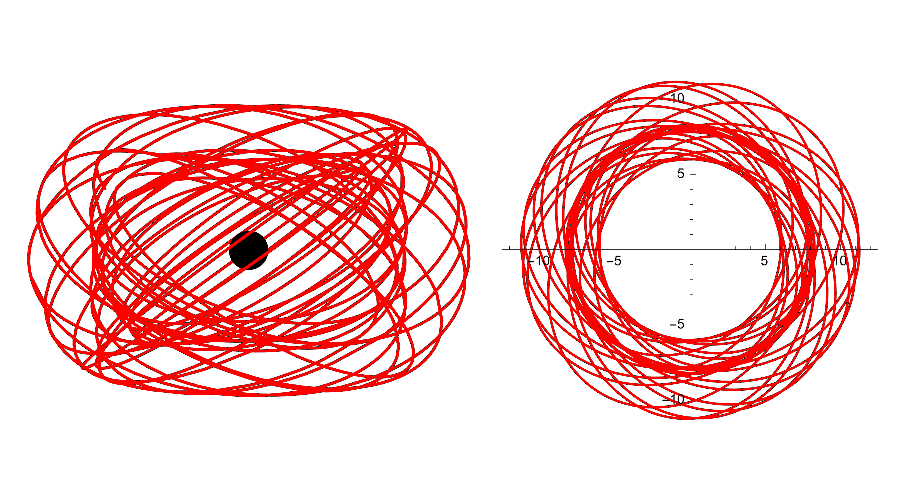
\includegraphics[width=0.85\textwidth]{images/resoTopSide.pdf}
    \caption[Resonant orbit example]{An example of a $(2,3)$ resonant orbit observed from the equatorial plane at $\theta=\pi/2$ (left), from above at $\theta=0$ (right). The parameter values for this orbit are $a=0.4$, $p=8.99834$, $e=0.2$, $x=0.8$.}
    \label{fig:resoexample2-3}
\end{figure}

\begin{figure}[!ht]
    \centering
    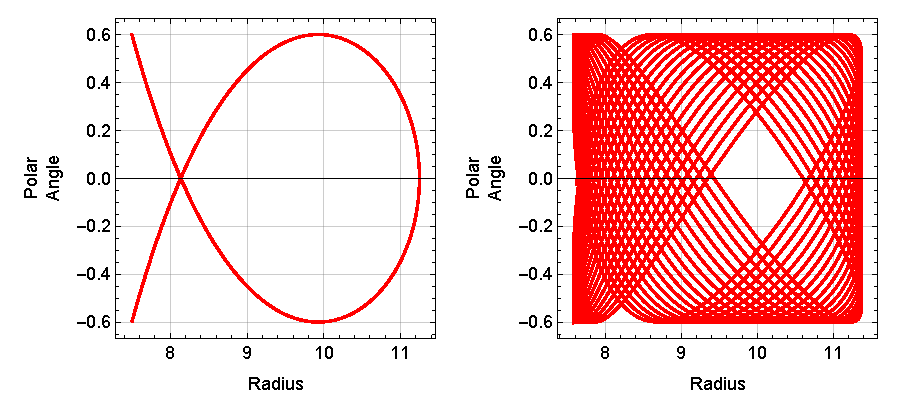
\includegraphics[width=0.85\textwidth]{images/resorThPlusPert.pdf}
    \caption[Two $(r,\theta)$ plots showing an unperturbed and a perturbed resonant orbit]{An $(r,\theta)$ plot of an unperturbed  $(2,3)$ resonant orbit (left), and an $(r,\theta)$ plot of the same $(2,3)$ resonant orbit where $p$ has been perturbed by $+0.1$ (right). The parameter values for this orbit are $a=0.4$, $p=8.99834$, $e=0.2$, $x=0.8$.}
    \label{fig:23ResoPerturb}
\end{figure}

Once Eqn.~\eqref{eqn:resCond} holds, meaning we have a resonant orbit, the path traced out in the orbit's $(r,\theta)$ plot will be closed, like the one seen on the left in Fig.~\eqref{fig:23ResoPerturb}, where the polar angle $\theta$ is plotted against the radius $r$.
A path has been carved out in the first full orbit, and there will be no deviation from this path for all time.
Due to this fact, there are areas of the $(r,\theta)$ plane that the orbit will never reach.
In contrast to this, if the same orbit in Fig.~\eqref{fig:resoexample2-3} is perturbed so that we have $(a,p,e,x)=(0.4,\;8.99834+0.1,\;0.2,\;0.8)$ the path traced on the $(r,\theta)$ plane will not repeat trivially, and instead the path will reach every point on the $(r,\theta)$ plane (over a long enough time period).
This can be seen in the plot on the right in Fig.~\eqref{fig:23ResoPerturb}.

\begin{figure}
    \centering
    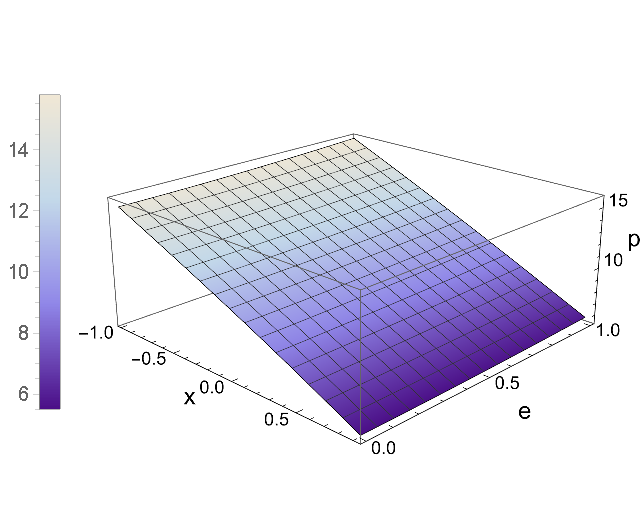
\includegraphics[width=0.5\textwidth]{images/pexplot.pdf}
    \caption[Plot of $p$-$e$-$x$ plane for resonant parameter values]{For fixed spin $a=0.9$, the above plot shows the value of $p$ required to achieve resonance given values of $x$ and $e$.}
    \label{fig:pexplot}
\end{figure}

\subsubsection{Extrapolation of resonant parameter values}
Taking the spin of the black hole fixed such that $a=0.9$ for the following analysis, we vary our values of $x$ and $e$ in the ranges $(-1,1)$ and $(0,1)$ respectively, and calculate the corresponding $p$ value that produces a resonant orbit, represented in Fig.~\eqref{fig:pexplot}.
Immediately we can see an apparently linear relationship between $x$ and $p$ for any fixed value of $e$.
It can be seen that for a resonant orbit with values $(p_0,e_0,x_0)$, if $x_0$ is increased by some value $\delta$, then to retain resonance, $p_0$ must be reduced by some value $k\cdot\delta$ to obtain new parameter values $(p_0-k\cdot\delta,e_0,x_0+\delta)$, and vice versa.
Under visual inspection, $e$ appears to have very little effect on the resonant value of $p$.
Therefore, we wish to interpolate between values at $e=0$ in the $p$-$x$ plane to create a linear approximation before extrapolating out for $e>0$.
This will create a set of $p$ values that could serve as a set of initial values for root-finding when calculating resonant orbits.
For the linear approximation we solve the equation $2\Upsilon_\theta=3\Upsilon_r$ for $(a,e,x)=(0.9,0,\pm 1)$, where $x=-1$ corresponds to the retrograde orbit and $x=1$ corresponds to the prograde orbit.
This problem corresponds to finding the non-asymptotic points of intersection in the graphs of Fig.~\eqref{fig:proretfreqs}, where the point of intersection for the prograde orbit is $p_\text{pro}=4.9626$ and the retrograde orbit is $p_\text{ret}=15.2677$.
A straight line of the form $\alpha+\beta x$ is calculated with coefficients $(\alpha,\beta)=(10.1152,-5.1525)$ and then extrapolated out to create the plane
\begin{equation}\label{eqn:planeequation}
    f(x,e)=10.1152-5.1525x+e.
\end{equation}
The error between the planes from Eqn.~\eqref{eqn:planeequation} and Fig.~\eqref{fig:pexplot} can be seen in Fig.~\eqref{fig:planeErr}.
We can see that there is a quadratic element to account for when we approximate using only a flat plane, and yet, the maximum error is only between $0.6$ and $0.7$.
Thus, we conclude that the plane produces values close enough to the true values that it can be considered a good method of approximation for resonant values in root finding.

\begin{figure}
    \centering
    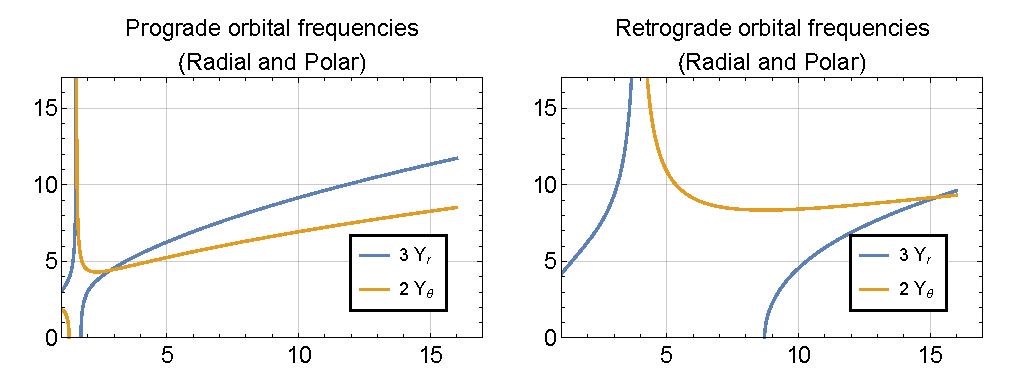
\includegraphics[width=0.9\textwidth]{images/proretfreqplots.pdf}
    \caption[Plot of radial and polar frequencies for prograde and retrograde orbits]{Plot of radial and polar frequencies for prograde (left) and retrograde (right) orbits, the points of intersection correspond to the $p$ value which produces a resonant orbit.}
    \label{fig:proretfreqs}
\end{figure}

\begin{figure}
    \centering
    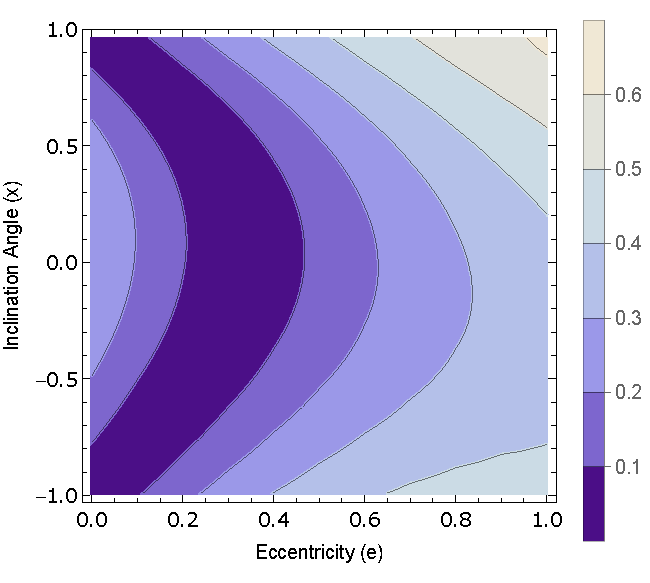
\includegraphics[width=0.5\textwidth]{images/planeErr.pdf}
    \caption[Contour plot of estimation error]{Contour plot showing the error between the true $p$ values to produce resonance and the values from our plane in Eqn.\eqref{eqn:planeequation} given a point $(e,x)$.}
    \label{fig:planeErr}
\end{figure}